\documentclass[10pt,twocolumn]{z2-article}
%\pagestyle{empty}

\usepackage{times, oneinchmargins}
\usepackage{setspace}
\usepackage[pdftex]{graphicx}
\usepackage{multirow}
\usepackage{amssymb}
\usepackage{alltt,url}
\usepackage{listings}
\usepackage{cite}
\usepackage{hyperref}
\usepackage{breakurl}
\usepackage{fancyvrb}
\usepackage{relsize}
\usepackage{soul}
\usepackage{array}
\usepackage{subcaption}
\usepackage{booktabs}
\usepackage{enumitem}

% Spacing stuff
\textwidth=6.5in
\textheight=9in
\lstset{basicstyle=\footnotesize\ttfamily,breaklines=true,captionpos=b, aboveskip=0pt, belowskip=3pt, abovecaptionskip=0mm, belowcaptionskip=0pt}
\setlength{\textfloatsep}{3pt}
\setlength{\abovecaptionskip}{2mm}
\setlength{\belowcaptionskip}{0pt}
\setlength{\dbltextfloatsep}{3pt}
\newlength{\tmpa}
\newlength{\tempa}

\begin{document}
\nocite{*}
\begin{spacing}{1.0}
\title{
     Uncovering Twilio: Insights into Cloud Communication Services
    }

\linespread{1.2}

\author{
  Ramnatthan Alagappan\\
  \texttt{ra@cs.wisc.edu}
  \and
  Sourav Das\\
  \texttt{souravd@cs.wisc.edu}
}

\date{\vspace{-0.2in}}
\maketitle




\section{Abstract}
\label{sec-abstract}

Cloud communication services are Internet-based voice and data communication service providers where telecommunications applications, switching and storage are hosted by a third-party outside of the organization using them, and they are accessed over the public Internet~\cite{wikicc}. 
Cloud communications providers deliver voice & data communications applications and services, hosting them on servers that the providers own and maintain, giving their customers access to the cloud. Because they only pay for services or applications they use, customers have a more cost-effective, reliable and secure communications environment, without the headaches associated with more conventional PBX system deployment.




\section{Introduction}
\label{sec-intro}





\section{Motivation and Related Work}
\label{sec-motivationandrelated}
Businesses want to delegate communication from their applications and services because of the advantages provided by CCS. The number of enterprises using CCS has seen a steady increase since its advent. Though there are no enough evidences that this pattern is going to continue, because cloud commucation services provide an attractive cost-model and easy-to-use APIs, we strongly believe that this trend is going to continue in the future. As more and more enterprises start using CCS like \textit{Twilio}, there is a good chance that this traffic may contribute to a good fraction of internet traffic in the future. \par
There have been lot of studies on VOIP service like \texit{Skype} in the past [1,2]. There have been recent studies on cloud storage service like \textit{Dropbox} [3]. Best to our knowledge, we are the first to study cloud communication services. Similar studies have been carried out previously - [3] provides a thorough characterization of the Dropbox protocol and traffic patterns. They provide insights into how traffic to \textit{Dropbox} varies across four different networks including home and campus networks. Our study on the other hand does not deal with traffic analysis since we did not have the sophistication of collecting the packet traces in the campus network. Our study aims at studying the architecture and protocols of the entire \textit{Twilio} ecosystem. Our study also aims at finding some possible enhancements to the entire \textit{Twilio} ecosystem. [1] provides a detailed packet level study of the \textit{Skype} protocol. The authors also provide deep insights into the \textit{Skype} architecture. Our study involves studying the architecture of the system and the protocols involved using a suite of gray box tools that we have developed. \par
The reminder of the paper is organized as follows. In secion 3, we provide a detailed analysis of the \textit{Twilio} ecosystem, architecture of the system, high level protocols for some key scenarios and packet level analysis for two scenarios. We give some detailed measurements with respect to call dequeuing rates in section 4. Then, we present some oddities that we found in the entire ecosystem in section 5. In section 6, we discuss some of the possible enhancements to the system. Finally we conclude by presenting the implications of our study and our future work.
\section{Twilio Overview}
\label{sec-twilioecoandprotocolstudy}
In what follows, we describe the Twilio Ecosystem, some of the possible scenarios using the Twilio APIs, the experimental setup that we used for our study, high level protocol study and then packet level protocol study.
\subsection{Twilio Ecosystem}
\label{subsec-twilioeco}
The Twilio ecosystem, as depicted in the Figure~\ref{fig:ecosystem} can be viewed as a layered architecture. In the bottom most layer lie the $Twilio$  $servers$. These servers lay the foundation of this ecosystem by exposing a set of data and voice communication APIs for sending and receiving voice calls and messages. 

In the middle layer, lie the $Application$ $servers$. These servers are installed by Twilio customers with dedicated Twilio accounts. For e.g. These application servers might belong to some company X that wants to provide VoIP service to its customer. Each Twilio account is linked to 1) one or more Twilio numbers, 2) an Account SID and 3) an Auth Token. A Twilio number is a ten digit phone number. Account SID is an unique identifier for a Twilio account. Auth Token is a token used by Twilio Servers to authenticate an account. The Application server uses the Account SID and Auth Token to access the Twilio APIs. The cost model for this second layer Application servers (or Twilio customers) is typically \textit{pay per message} or \textit{pay per call}. 

In the top most layer, lie the $Clients$ which could be browser based clients or phone based clients. An important thing to note here is that these Clients are $not$ the direct customers of Twilio, instead they are the customers of the services that are built on top of Twilio. For e.g. These clients could be the customers of company X that is providing VoIP service. These clients, can be free customers or paid customers of company X. Also, depending on the type of service that the layer two based Twilio customers wants to provide, it is possible that these layer three is non-existent.  The Clients when present, in order to use the services and communicate with each other need to register with the layer three Twilio servers. This is done using a \textit{capability token} which is provided by the Application Server. 

So far we have only discussed how the Twilio clients connect to each other in the Twilio ecosystem. The Twilio clients and the Application servers can also interact with the external phones belonging to different carriers via the Twilio servers. Hence, these external phones also form a part of the Twilio ecosystem.

\begin{figure}
\centering
%\begin{minipage}{.45\textwidth}
  \centering
  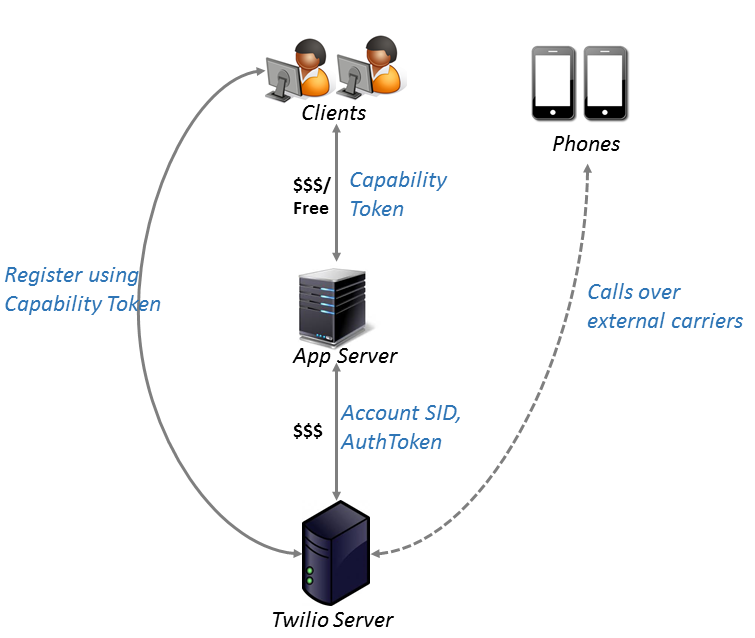
\includegraphics[width=0.45\textwidth]{figs/Ecosystem.png}
  %Mazu_frame_new.png}
\caption{Twilio Ecosystem}
\label{fig:ecosystem}
\end{figure}     



\emph{Application Container: } Each Twilio number is linked to an application container. The application container contains two URLs: $Voice URL$ and $Message URL$. These URLs are configurable and are usually configured by the Application server administrators (or Twilio customers). Whenever an incoming call or message for a Twilio number arrives, the Twilio server makes post request to these URLs. The content generated by these URLs direct Twilio servers to perform the needed actions on the incoming calls or messages. These contents are in form of a special markup language called $TwiML$ described in the subsequent section. Additionally, Twilio appends the \textit{query parameters} that it obtains from the end-clients before making the requests to the application servers. 
 \begin{figure}
 \centering
 %\begin{minipage}{.45\textwidth}
   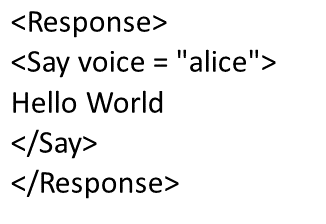
\includegraphics[width=0.25\textwidth]{figs/TwiML.png}
 \caption{Sample TwiML Snippet}
 \label{fig:TwilML}
 \end{figure} 
\begin{figure*}[t!] 
\centering
%\begin{minipage}{.45\textwidth}
  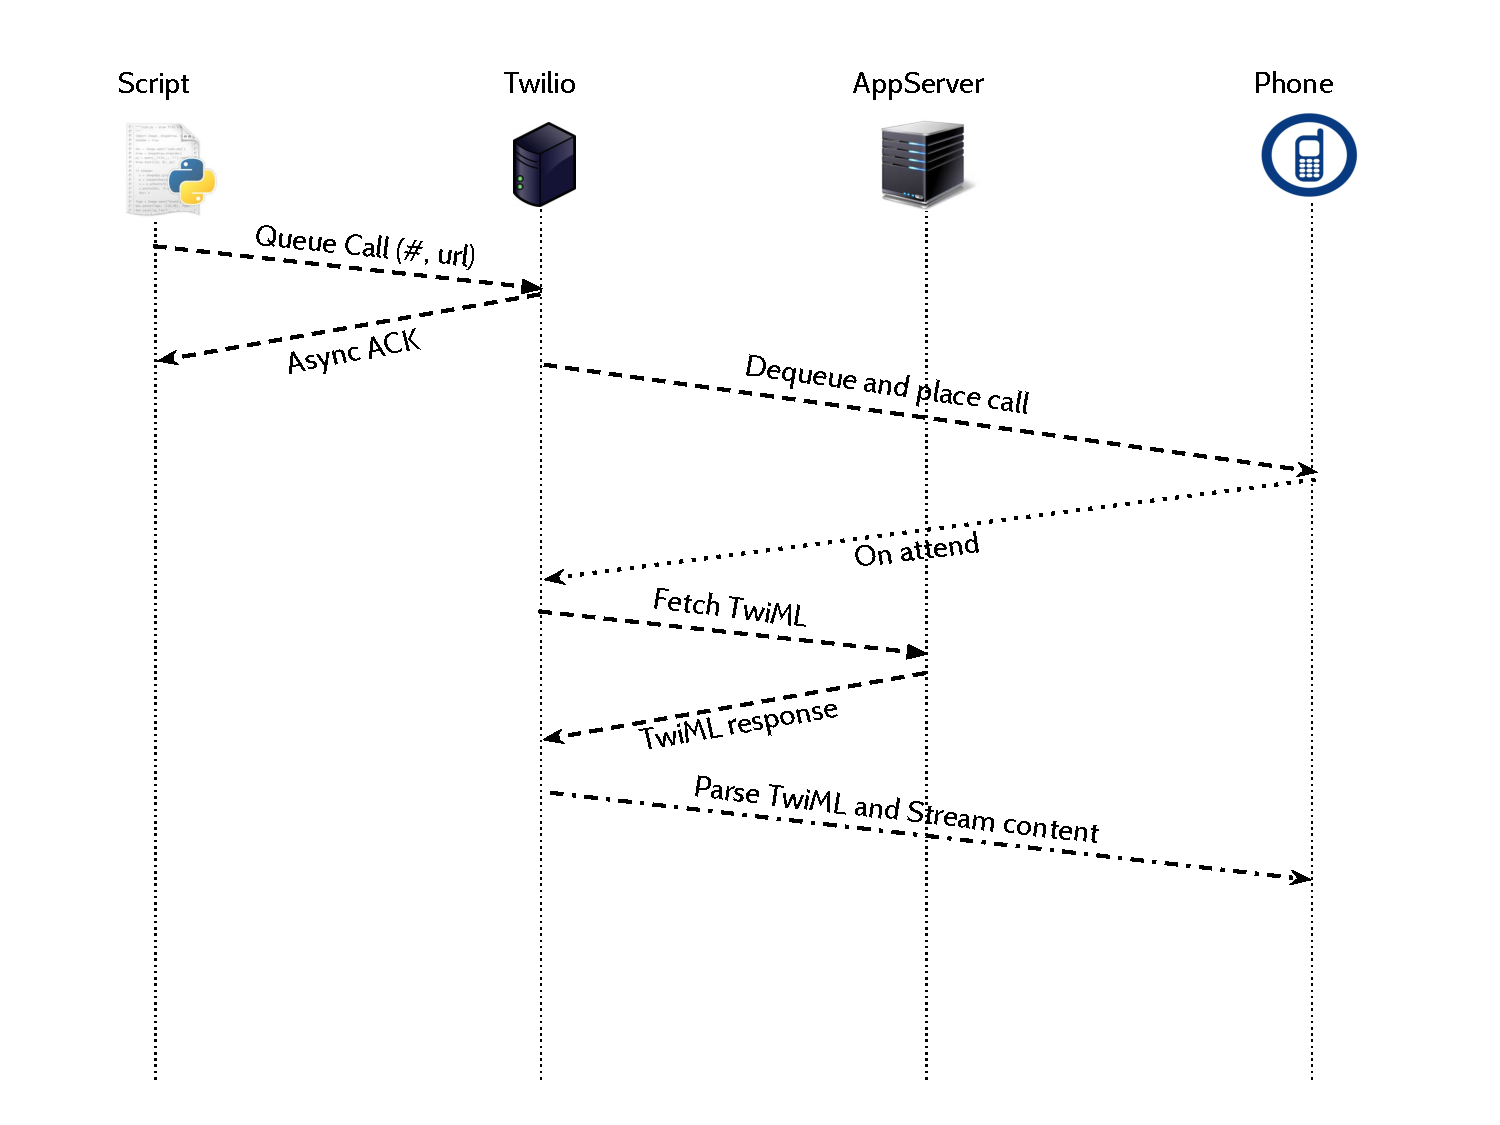
\includegraphics[width=0.8\textwidth]{figs/auto.pdf}
\caption{Automated call to a phone}
\label{fig:autocall}
\end{figure*} 

\emph{TwiML:  } It is a markup language developed by Twilio. It contains a set of simple verbs that can be used by the Application Servers to direct the Twilio servers about the action that needs to be taken whenever a call or message is received to its number. Various kinds of verbs are supported as shown below which can be used to create interactive applications atop Twilio.
\begin{itemize}
\item Say - Read text to the caller 
\item Play - Play an audio file for the caller
\item Dial - Add another party to the call
\item Record - Record the caller's voice
\item Gather - Collect digits the caller types on their keypad
\item Sms - Send an SMS message during a phone call
\item Hangup - Hang up the call
\item Queue - Add the caller to a queue of callers.
\item Redirect - Redirect call flow to a different TwiML document
\item Pause - Wait before executing more instructions
\item Reject - Decline an incoming call without being billed
\end{itemize}

For e.g. The TwiML snippet shown in Figure~\ref{fig:TwilML} will say Hello World (dictated by the verb "say") to the caller in female voice (dictated by the attribute "voice"). Our experience with TwiML suggests that it is very simple to use and powerful with respect to the diversity of verbs that it supports.



\subsection{Scenarios}

There are multiple scenarios that one can enable with the help of Twilio Apis. Some of them are:

\begin{itemize}
\item $Automated$ $calls: $ Twilio APIs can be used to place automated calls to phone numbers to deliver a pre-recorded message.
\item $Voice$ $calls: $ VoIP applications can be built atop Twilio voice APIs which can be used to place voice calls. There are three scenarios possible for VoIP applications:  
\begin{itemize}
\item Call between VoIP Clients
\item Call from Phone to VoIP Client
\item Call from VoIP Client to Phone
\end{itemize}
\item $Messages: $ Twilio message APIs can be used to send automated messages.
\end{itemize}
\emph{\textbf{Voice calls between VoIP clients:} }
\begin{figure*}[t!] 
\centering
%\begin{minipage}{.45\textwidth}
  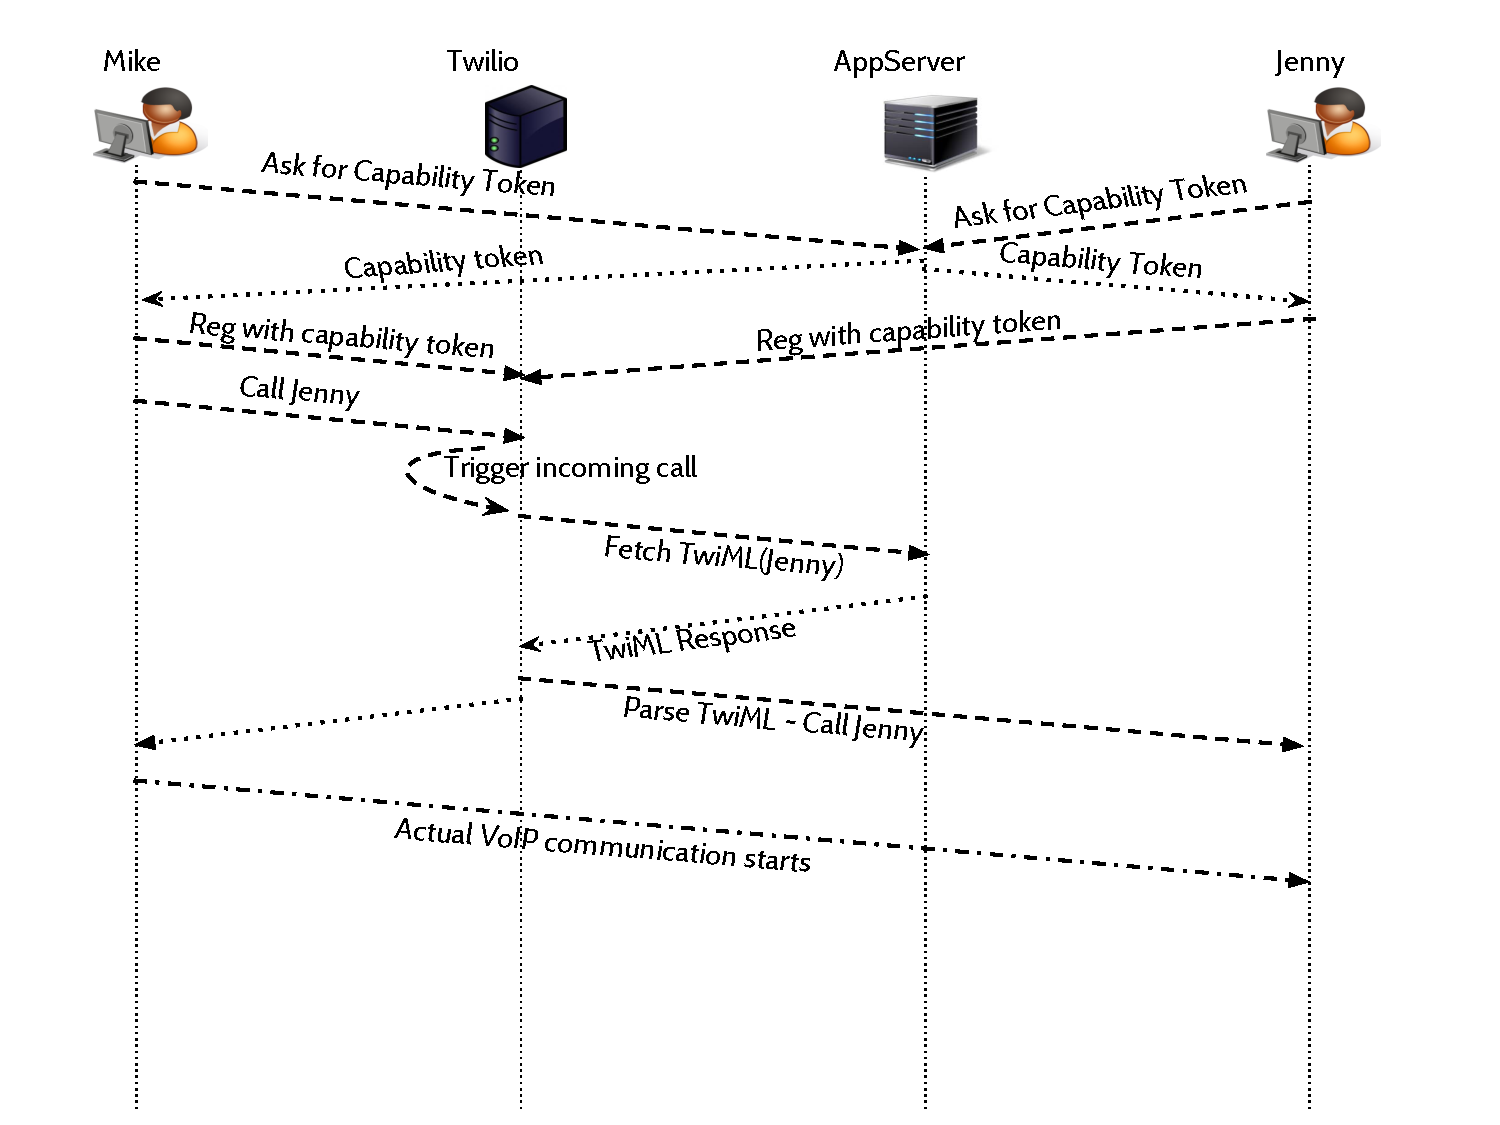
\includegraphics[width=0.8\textwidth]{figs/twoclients.pdf}
\caption{Call between two VoIP clients}
\label{fig:2VoIPcall}
\end{figure*}
\subsection{Experimental Setup}

For our study, we developed a simple VoIP service (called VoT) atop Twilio and deployed it on OpenShift RedHat Cloud. The VoT server also hosts a simple web interface which can be used to place voice calls by specifying a phone number or the registered names of VoIP clients. For making automated calls and sending automated messages we have developed python scripts using the Twilio client libraries which directly calls into the Twilio APIs. For our study, we extensively use traces collected at different places. This includes application level trace messages collected at our VoT server, logs in Twilio user portal, Twilio object store queries and \textit{Wireshark} traces collected at client machines.

\subsection{High Level Protocol Study}
\label{subsec-protostudy}
We now present a high level protocol study of some of the important scenarios that Twilio supports. 

 
\begin{figure*}[t!] 
\centering
%\begin{minipage}{.45\textwidth}
  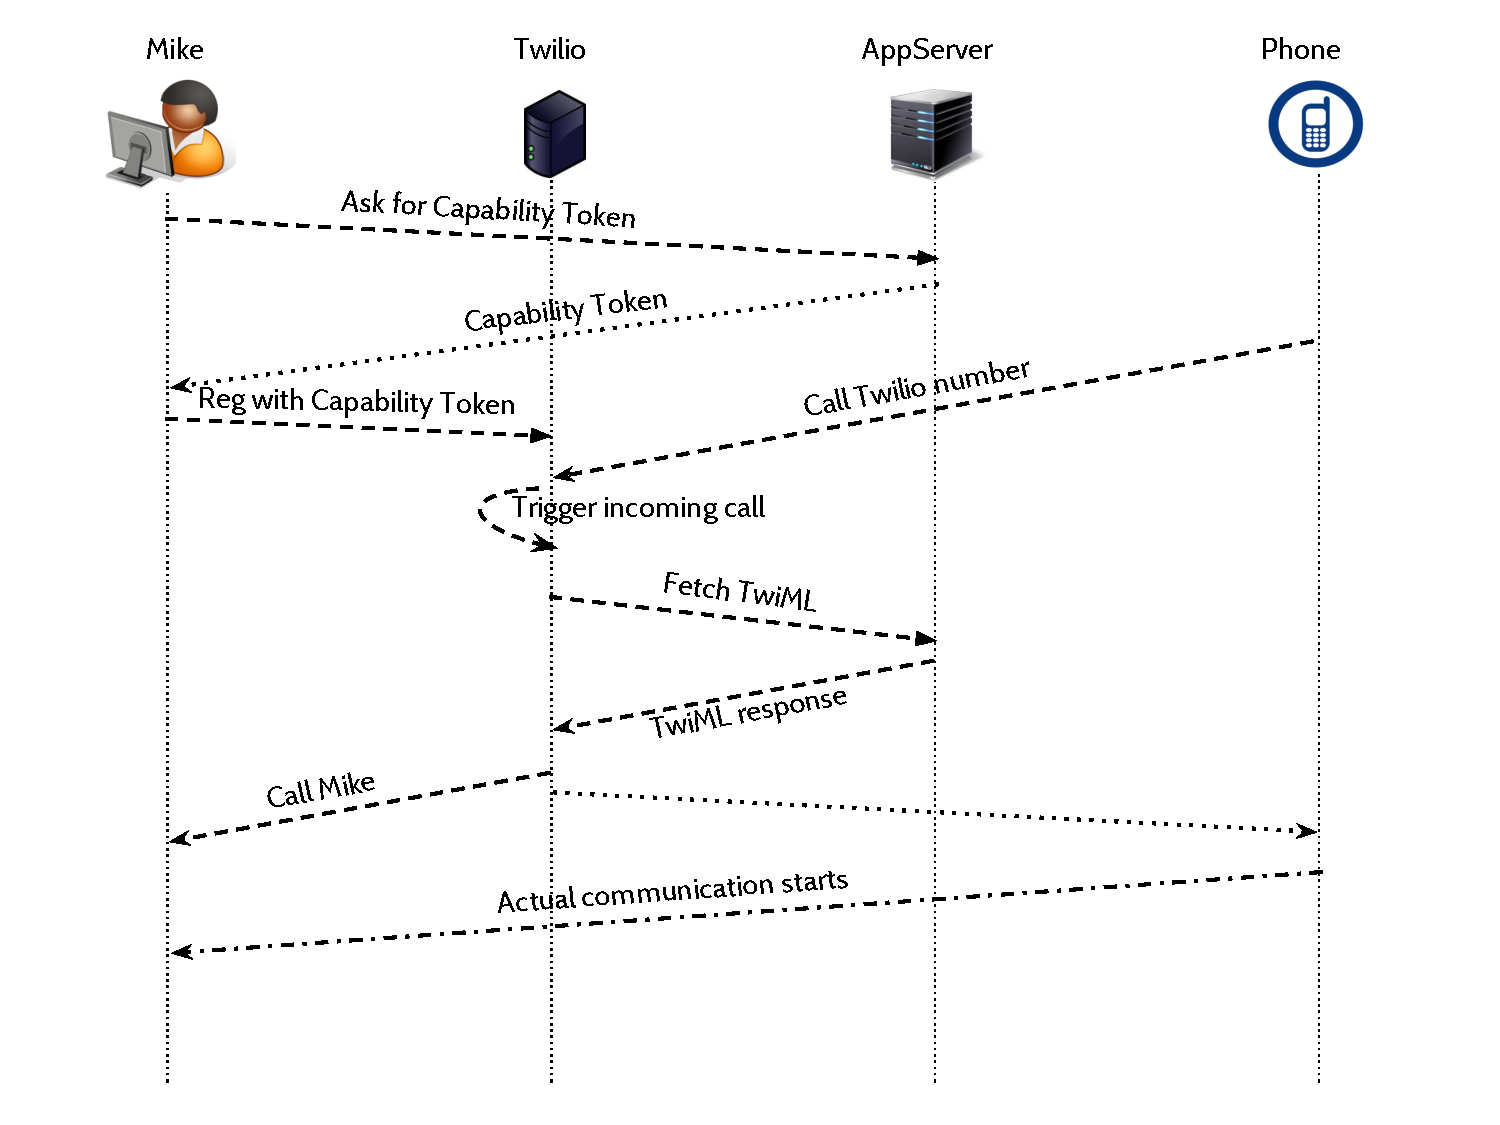
\includegraphics[width=0.8\textwidth]{figs/p2c.pdf}
\caption{Call from phone to a VoIP client}
\label{fig:callfromphone}
\end{figure*}

\emph{\textbf{Automated calls to phones:} }
The protocol diagram for this scenario is shown in  Figure~\ref{fig:autocall}. At first, a script (our python script) queues a call request specifying the phone number to which the call needs to be placed and an url indicating the location of the TwiML response. The Twilio server acknowledges the request and places the call. Once the phone attends the call, the Twilio server does a \textit{HTTP POST} or \textit{HTTP GET} to the url in the call queue request to fetch the TwiML response. In our experiments, we hosted these pre-recorded messages in our application servicer. The application server processes the request and sends a TwiML response in return. The Twilio server parses the TwiML response and finally streams the content to the phone.  

\emph{\textbf{Voice calls from phone to VoIP clients:} }
The protocol diagram for this scenario is shown in Figure~\ref{fig:2VoIPcall}. Let us say, Mike and Jenny are the two VoIP clients and Mike wishes to call Jenny. As shown in Section~\ref{subsec-twilioeco}, for Mike and Jenny to communicate they need to first register with the Twilio Server. Hence, Mike and Jenny at first request the Application server for capability tokens. Once the Application server delivers the tokens, Mike and Jenny register with the Twilio server using the tokens. Mike then queues a call to Jenny. An interesting thing to note here is that the Twilio server does not have information about what to do with the call. It need to communicate with the Application server to get this information. For this, it triggers an incoming call to the Twilio number to which Mike is linked to. As stated in Section~\ref{subsec-twilioeco}, every incoming call to a Twilio number generates a post request on the voice URL present in the application container linked to that number. This post request is directed to the Application server with query parameter as "Jenny". The Application server parses the request and generates the appropriate TwiML content indicating the action that needs to be taken. In this case, the application server would serve a response that contains a \textit{Dial} verb and the client for the \textit{Dial} verb would be "Jenny". The Twilio Server parses the TwiML and places a call to Jenny. Finally, Mike is notified about this and the voice communication starts. Note that the actual voice communication is $not$ peer-to-peer and is routed via Twilio servers.  

\emph{\textbf{Voice calls from VoIP clients to phone:} }
The protocol diagram for this scenario is not shown for space constraints and is similar to that shown in Figure~\ref{fig:2VoIPcall} except that Jenny has a dedicated phone number and hence does not need to register with the Twilio server. Lets say, Mike is a VoIP client and Mike wishes to call Jenny with a dedicated phone number (may belong to any carrier). Mike will at first request the Application server for a capability token. Once the Application server delivers the token, Mike will register with the Twilio server. Mike then places a call to Jenny's number. As in the case of two VoIP clients in the previous section, the Twilio server communicates with the Application server to get the information about the action that needs to be taken for the queued call. For this, it triggers an incoming call to the Twilio number linked with Mike. This incoming call generates a post request on the voice URL present in the application container. This post request is directed to the Application server with query parameter as "Jenny's phone number". The Application server parses the request, generates the appropriate TwiML content for the action that needs to be taken and delivers it to the Twilio server. The Twilio Server parses the TwiML and places a call to Jenny's phone. Finally, Mike is notified about this and the actual communication starts. 

\emph{\textbf{Voice calls from phone to VoIP clients:} }
The protocol diagram for this scenario is shown in Figure~\ref{fig:callfromphone}. Lets say, Mike is a VoIP client and a phone wishes to call Mike. Mike will first request the Application server for capability token with incoming capability. Once the Application server delivers the token, Mike registers with the Twilio server. When the phone calls the Twilio number associated with Mike, the Twilio server triggers an incoming call to that Twilio number. The incoming call generates a post request on the voice URL present in the application container. This post request is directed to the Application server. The Application server parses the request, generates the appropriate TwiML content for the action that needs to be taken and delivers it to the Twilio server. For our study purpose, whenever there is a call from a phone, the application server instructs Twilio through TwiML to forward the call to a pre-determined client name. In this case, the pre-determined name is Mike. The Twilio Server parses the TwiML and places a call to Mike. Finally, the phone is notified about this and the actual communication starts.

\subsection{Packet Level Analysis}
In this subsection, we dig deeper and present the packet level analysis for a scenario where a browser makes a voice call to a phone or another browser based client. 
%We also show another message level analysis for automated message sending scenario in section \ref{sec-oddities}. 

\begin{figure*}[t!] \centering
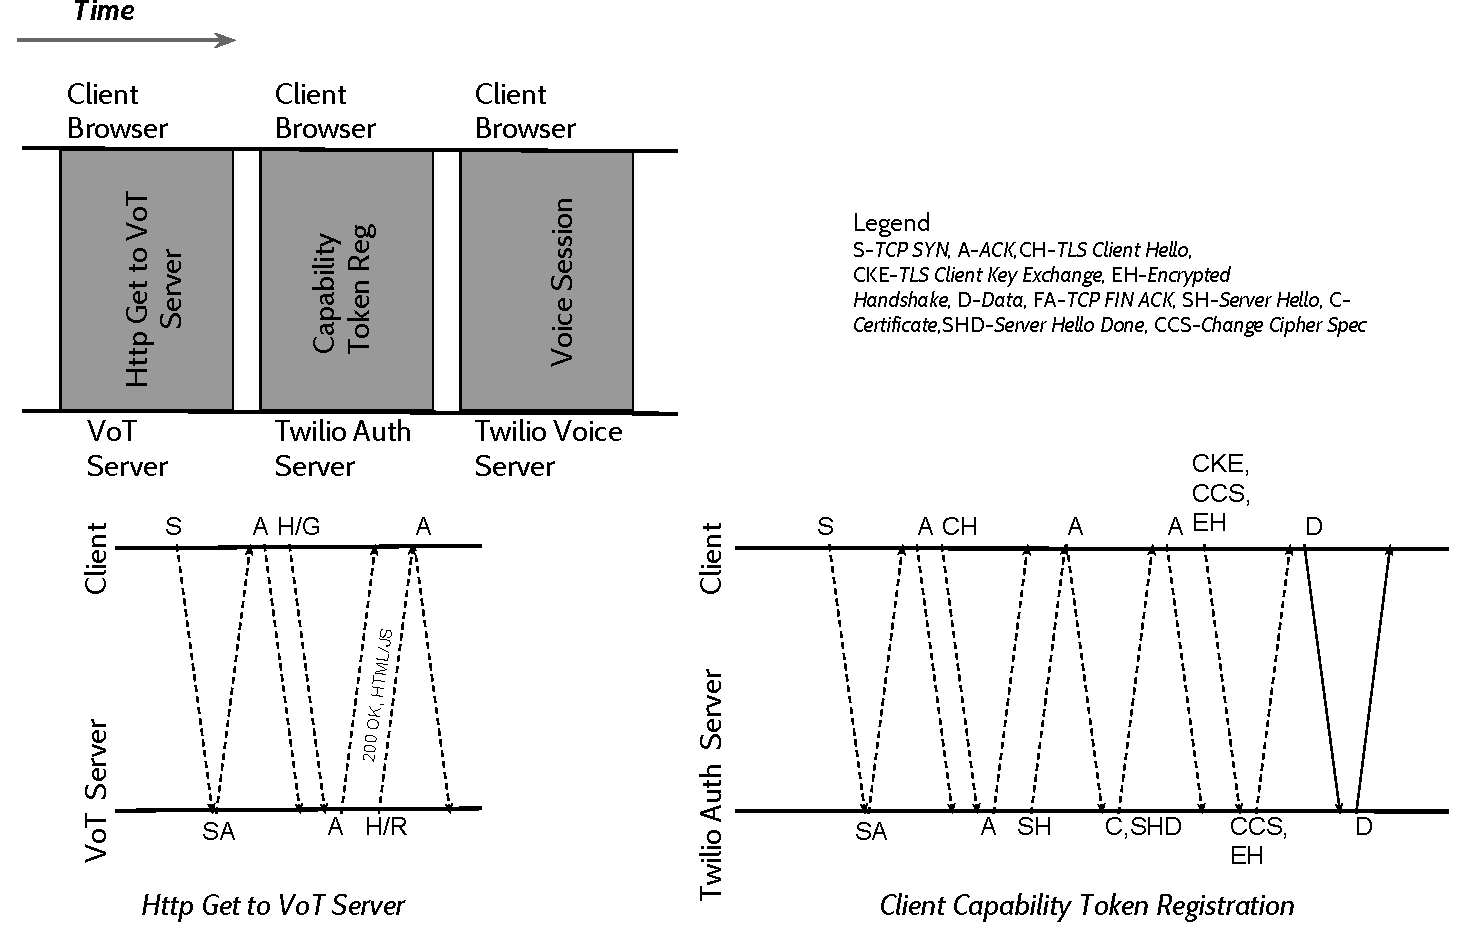
\includegraphics[width=\textwidth]{figs/voicecallpacketlevel.pdf}
\caption{\textbf{Voice Call from Browser Client} {\footnotesize\textit{
The figure shows sequence of packet exchanges that happen between the client and other components of the system. The top diagram shows the high level operations. The participants are shown above and below the top and bottom lines. The left bottom figure shows how the client interacts with the application server to obtain the \textit{capability token} and it corresponds to the first block in the top diagram. The right bottom diagram shows the sequence of messages exchanged between the client and the \textit{Twilio} server when the client executes the \textit{Twilio.Device.Setup} method and corresponds to the second block in the top diagram.  
}}}
\label{fig:messagelevel}
\end{figure*}

Figure~\ref{fig:messagelevel} shows the sequence of events that happens when a browser based client wants to make a VoIP call to another browser based client or a phone. As shown, at first the client browser does a \textit{HTTP GET} request to the application server that we have deployed. The application server generates a \textit{capability token} and passes it onto the client. The client side javascript includes the \textit{twilio javascript} library and does \textit{Twilio.Device.Setup} to register its capability with the \textit{Twilio} servers. The sequence of messages for the second block is also shown. The client passes the \textit{token} as \textit{HTTP} data after establishing a TLS session with the server. After this step, the client is free to make a call to either a phone number or another browser based client. The actual voice communication is tunneled through \textit{Twilio} servers and it involves \textit{RTMP} protocol. This sequence of packet exchanges are not shown due to space constraints. 

\section{Measurements}
\label{sec-measurements}

In this section, we provide measurements with respect to call and message dequeuing rates. \textit{Twilio} provides guarantees that the placed calls and messages will be dequeued at a rate of 1 per sec and placed onto the phones or the browser clients ~\cite{guaranteelink}. We measure the degree to which this guarantee is met. All the experiments were conducted on Lenovo W530 laptop with 8 GB RAM running on 4 cores connected to a 30 Mbps Internet link.

\subsection{Calls}
\label{sec-measurements-calls}
We developed scripts that can queue automated calls to US phones and online browser clients. We queue the first call to the browser client and queue a variable number of calls to a US phone and then finally place one more call to the browser client. \textit{Twilio} dequeues the calls in the order it was placed into the queue. Using \textit{Wireshark} in the browser client, we collect the packet traces and the timestamps of the incoming call connections. We then calculate the time difference between the first call and the second call received by the browser. A careful reader would note that the call timestamps may not reflect the actual time when the call was dequeued from the queue and it will include the network latency involved in placing the call to the browser client. We noticed that this latency was lesser than 50 ms and so was discounted for the purpose of our calculations. 

\begin{figure} \centering
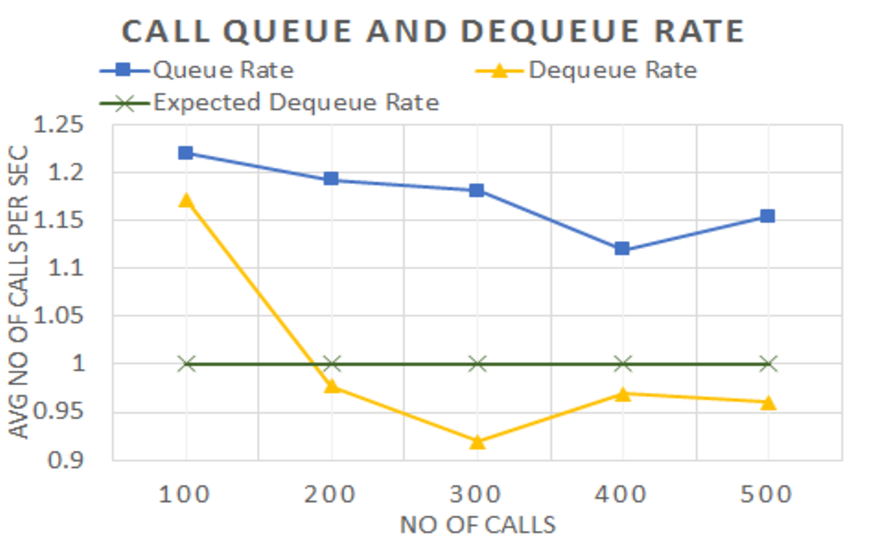
\includegraphics[width=0.45\textwidth]{graphs/calls.pdf}
\caption{\textbf{Calls queuing and dequeuing.} {\footnotesize\textit{
The figure shows the queuing and dequeuing rate for calls
}}}
\label{fig:calls}
\end{figure}

Figure~\ref{fig:calls} shows the expected dequeue rate, observed dequeue rate and queue rate for calls. The horizontal axis shows increasing number of calls that we place to the phone and the vertical axis shows the queue or dequeue rate. As mentioned before \textit{Twilio} gives a guarantee to dequeue calls at the rate of 1 per second. This is shown by the flat line. We define the queue rate as the rate at which the client library can place calls into the \textit{Twilio} call queue. It is quite possible to achieve higher values of queue rate with high speed links. This value does not necessarily imply that the \textit{Twilio} server has a throttling mechanism for adding calls into the queue. The \textit{Dequeue rate} line shows the observed dequeue rate in our experiments. We notice that for a small number of calls such as 100, \textit{Twilio} dequeuing mechanism performs really well than expected. As the number of calls increases, the dequeue rate drops slightly below 1 but stays between 0.9 and 0.95. We believe that this behavior is completely acceptable if further increasing the number of calls to say few thousands still does not reduce the dequeue rate. 

\textit{Summary}. \textit{Twilio} call dequeuing guarantees are met and exceeded for small number of calls like 100. The dequeue rate slightly falls below 1 as the number of calls increases beyond 100. If applications need very critical and real time data to be delivered to phones or clients, we believe it is advisable to use one Twilio number for say around 100 outgoing client/phone connections. For applications that do not need this level of delivery accuracy, we believe this behavior is completely acceptable. 

\subsection{Messages}
\label{sec-measurements-sms}
We developed scripts that can queue automated messages to US phones. We queue 100 messages with varying message sizes to a sinlge US phone number. \textit{Twilio} dequeues the messages in FIFO order similar to calls. We noticed that telephone networks take a very variable amount of time to deliver messages to phones. So, for calculating the dequeuing rate, we used the timestamps present in the \textit{message resource} in the \textit{Twilio} object store. We query these message resources using the REST APIs and arrive at the dequeue rate by looking at the \textit{sent timestamp} in the message resource.   

\begin{figure} \centering
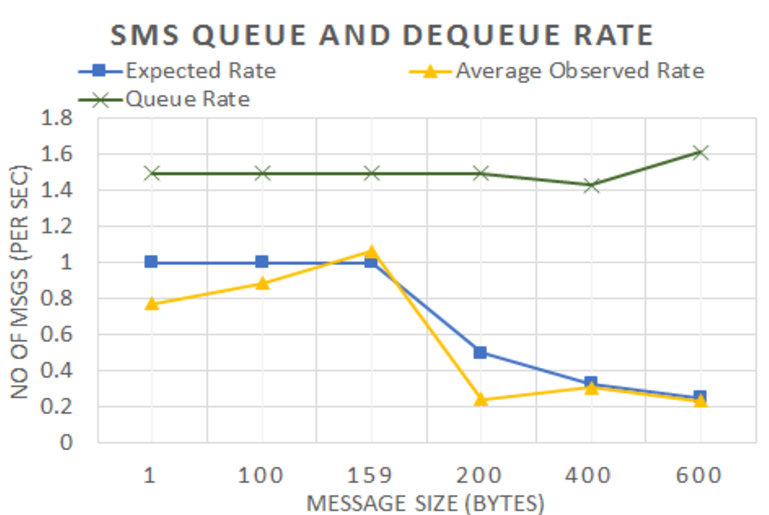
\includegraphics[width=0.45\textwidth]{graphs/sms.pdf}
\caption{\textbf{SMS queuing and dequeuing.} {\footnotesize\textit{
The figure shows the queuing and dequeuing rate for messages
}}}
\label{fig:sms}
\end{figure}

Figure~\ref{fig:sms} shows the expected dequeue rate, observed dequeue rate and queue rate for SMS. The horizontal axis shows increasing size of the messages that we place to the phone and the vertical axis shows the queue or dequeue rate. As mentioned before \textit{Twilio} gives a guarantee to dequeue SMS at the rate of 1 per second. Similar to Section \ref{sec-measurements-calls}, the queue rate shows the rate at which the client can push messages into the queue. It is interesting to note that the expected rate itself drops as the message size increases. \textit{Twilio} treats a single message as just 160 bytes. If the message contains say 170 bytes, \textit{Twilio} considers this as two messages and so it can queue at the rate of one message per two seconds and so the expected rate falls from 1 to 0.5. Similarly for a 400 byte message, there are three such chunks and so the expected rate drops to 0.33. It can be noted that the observed rate closely follows the expected rate. 

\textit{Summary}. \textit{Twilio} message dequeuing guarantees are well maintained. An interesting observation is that naive developers who do not notice the size limits of the messages may wrongly believe that \textit{Twilio} can dequeue at a rate of 1 message per second irrespective of the message size. We bring this out clearly in our study by showing that the expected rate itself falls down as the message size increases. 





\section{Oddities}
\label{sec-oddities}

We now present some of the oddities in the \textit{Twilio} ecosystem that we discovered during our study. First, as dicussed in section \ref{sec-twilioecoandprotocolstudy}, \textit{Twilio} charges twice for making a single outgoing call. We discovered this from the call logs available in the Twilio user portal. On first seeing this, we thought this was problem in the VoIP service code that we developed. But it turns out that even after using the code examples from Twilio developer forums, we were still observing this behavior. It should be noted that we built our VoIP service on top of a single \textit{Twilio number}. Second, we noticed that some applications may require \textit{ordered} message delivery for the messages that they try to send through \textit{Twilio} APIs. For example, a message based query system will require that the messages sent are delivered to the mobile phone in the same order. We understand that the telephone service provider can also reorder messages when delivering them. We understand that \textit{Twilio} does not provide any guarantee as such for ordered message delivery. But we wanted to measure to what extent the messages can be reordered. 

\begin{figure*}[t!] \centering
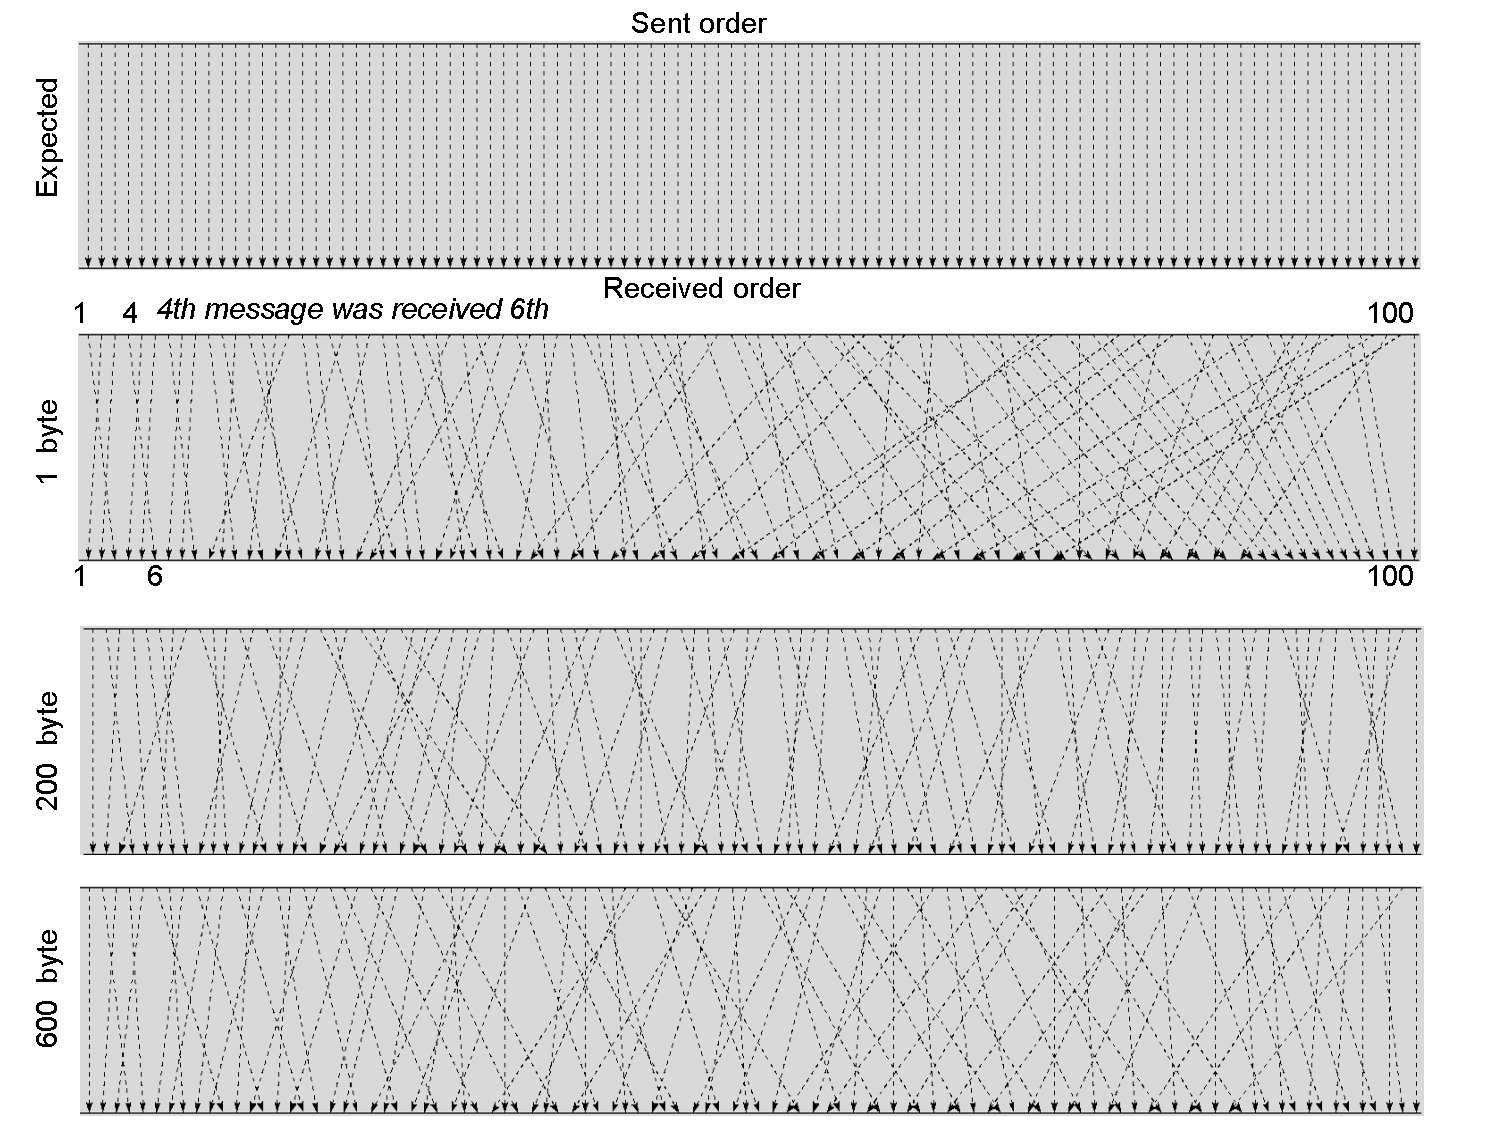
\includegraphics[width=\textwidth]{figs/reordering.pdf}
\caption{\textbf{SMS reordering} {\footnotesize\textit{
The figure shows the extent to which messages can get reordered. The top line in each strip denotes the sent order and the bottom line denotes the received order. The top most strip shows the ideal message delivery behavior. The second strip shows the reorderings that happened when 100 one byte messages were sent. The third strip shows the same for 200 byte messages and the last strip for 600 byte messages. Note that the sent time is identified from the \textit{sent timestamp} from the resource store so it represents the time for nearest upstream telephone carrier network to acknowledge the message was received and will be sent to the phone. 
}}}
\label{fig:reordering}
\end{figure*}


Figure {\ref{fig:reordering}} shows the message reorderings that can happen. It is understandable that \textit{Twilio} does not itself provide ordered message delivery. Application developers who develop on the \textit{Twilio} platform should be aware of this and should use suitable application level techniques to solve this issue. For example, the application use a label denoting the position of the message in the sequence. 

Third, we injected few faults into some parts of the system and observed how \textit{Twilio} reacts to these corner cases. For example we tested cases where in the \textit{TwiML} response returned by out VoIP server was malformed, unacceptably large, corrupted etc. We noted that the fault handling mechanisms were not uniform across all error scenarios. For example, if the \textit{TwiML Say verb} contained content greater than 4096 bytes, the call was placed but an error message was delivered to the attendee. On a different scenario when there are nested \textit{say} verbs in the \textit{TwiML} response, then a blank call was placed to the attendee. We are barely scratching the surface in terms of fault injection. We strongly believe that much better extensive techniques can be developed to analyse all the possible error conditions in the service.  

Fourth, during our study we observed a weird behavior in the \textit{Twilio Python client v3.66} library. We observed that when a client script tried to queue a call or a message using the \textit{create()} API, there was a HTTP level auth failure that was happening before the actual sequence of packets that were happening between the client and the \textit{Twilio} server. On further investigation and debugging, we found that the client was not passing the \textit{Auth Token} and \textit{Account SID} when the first REST API call is made to the server. Then the exception is handled and then the required credentials are passed onto the server for the subsequent REST API calls. We noted that this unwanted auth failure wastes 6 RTTs. We also believe that this can be easily optimized in the client library. 

\begin{figure*}[t!] \centering
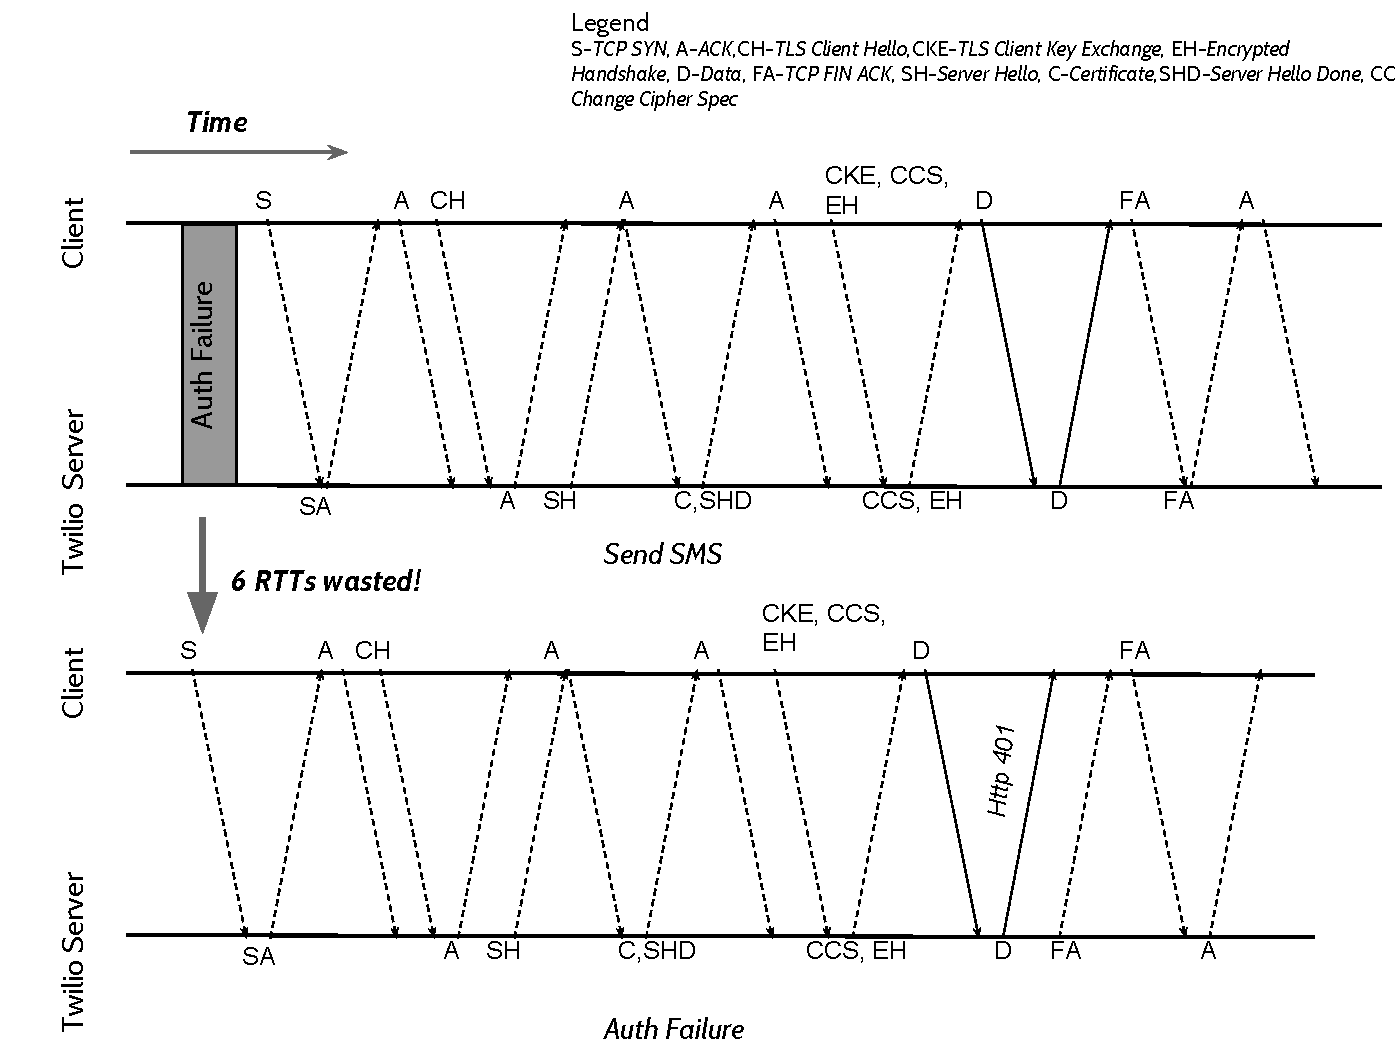
\includegraphics[width=\textwidth]{figs/authfailure.pdf}
\caption{\textbf{Packet analysis for creating automated SMS} {\footnotesize\textit{
The figure shows the sequence of packets exchanged between the client and the server when the client script tries to create a message.
}}}
\label{fig:authfailure}
\end{figure*}

Figure {\ref{fig:reordering}} explains this client library behavior. 
\section{Discussion}
\label{sec-discussion}
We now discuss some possible enhancements to the entire \textit{Twilio} ecosystem. 

\emph{\textbf{Client Library Improvements:}}
We showed that the client library can be optimized to save few RTTs in the previous section. It is important to notice that we identified this just by manually studying the behavior of the client library. We believe that there should be more robust and extensive ways to study the client's interaction with the server. We also showed in the previous section that fault handling mechanisms are not uniform across the system spanning the service and the client library. Also, in most of the cases that we tested by inducing faults from the caller side, we found that the callee is notified of the error conditions instead of caller. We believe that, in such scenarios it is best to inform caller with consistent error notifications since it is the caller who can take actions against those error and correct the errors.


\emph{\textbf{Security:}} We found that presently there is no way for Application servers to authenticate the Twilio servers when the later makes the \textit{HTTP POST} requests. In the interest of securing the application servers from attacks, we believe Twilio may provide IP whitelists which can be used by the Application servers to authenticate requests. Even IP whitelists might not be sufficient for scenarios in which Application servers are located behind proxies and the IP from which request originates gets masked (e.g. application server hosted behind load balancer in PaaS architecture). For such scenarios some more robust security measures needs to be provided.

\emph{\textbf{Intelligent TwiML fetching:}} As we have shown in Section~\ref{subsec-protostudy}, in case of automated calls to phone, Twilio server fetches the TwiML only after placing the call. We understand that this technique saves extra RTTs in case the call is rejected by the phone. But from the perspective of a callee and assuming that most calls will be answered, we believe it is best to prefetch TwiML before placing the call. Also, we see that in the current automated call model the application server is contacted each time a call is placed. One of the most popular use of automated call is to send/broadcast a single message to multiple numbers (e.g. to send promotional messages or alerts). In such scenarios, it is wasteful to flood the application server to fetch the same content multiple times both from Application server as well as Twilio server point of view. To handle such scenario Twilio might provide some special options using which the application server can indicate that the same message has to used for a specified number of calls or for some specified period of time and the Twilio server can then fetch the request once and cache it.   
 
\section{Future Work and Conclusions}
\label{sec-futureandconclusion}

In this section we discuss some of the possible avenues to extend this work, then present the implications of our study and finally conclude. As a future work, we think to study other CC services and compare different services in terms of traffic characters, usage patterns, user base diversity etc. We also intend to develop a much more generic and sophisticated gray-box framework to study CC services. Our current implementation of the toolbox is highly specific to \textit{Twilio}. We also started looking at the security aspects of the \textit{Twilio} servers by doing port scans using \textit{nmap}. From our initial analysis, the servers have only ports 80 and 443 open. As a future work, we would like to analyse if some impersonation attacks are possible with \textit{AuthTokens}. We also want to study how misbehaving clients can attack or cause some form of interference in the system.

Our study has implications for both application developers and \textit{Twilio} developers. First, we showed different components of the \textit{Twilio} ecosystem and how they interact. Our study gives more insights for developers to build robust applications atop \textit{Twilio} platform. We also showed how \textit{Twilio} meets its guarantees in terms of call and message dequeuing rates. This gives the application developers a good sense of what to expect from the \textit{Twilio} service. Second, we should some possible improvements to \textit{Twilio} in sections \ref{sec-oddities} and section \ref{sec-discussion}.

To conclude, we developed a simple VoIP service atop \textit{Twilio} platform and a graybox toolset to gain insights in to the protocols and the architecture of the system. We also empirically measured call and message queue/dequeue rates. We showed some interesting oddities in the service and the client library. We also pointed out to some possible enhancements to the \textit{Twilio} ecosystem. We showed that our study has implications for both application developers and \textit{Twilio} developers. Our study is a small step towards studying the rapidly growing Cloud Communication Services arena and we strongly believe further research is required in exploring this area. 
%\clearpage Remove comment if you want references in a separate page
{ \footnotesize
   %\bibliographystyle{alpha}
   %\bibliographystyle{abbrv}
   \bibliographystyle{plain}
   %\bibliographystyle{unsrt}   

   \bibliography{references}
   %\bibliography{swami}
}

% {\scriptsize  is the smallest

\end{spacing}
\end{document}

